documentclass[class=minimal,border=0pt]{standalone}
\usepackage{tikz}
\usetikzlibrary{calc}
\begin{document}
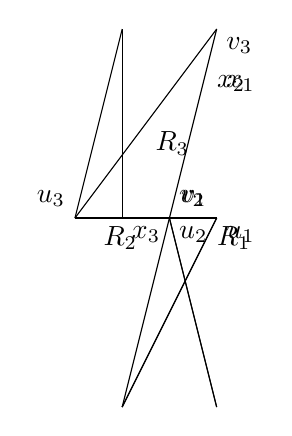
\begin{tikzpicture}[scale=.6]
% vertices
\coordinate (a) at (1,4);
\coordinate (b) at (-1,4);
\coordinate (c) at (1,-4);
\coordinate (d) at (-1,-4);
\coordinate (e) at (-2,0);
\coordinate (f) at (-1,0);
\coordinate (g) at (0,0);
\coordinate (h) at (1,0);

% edges
\draw (a)--(d);
\draw (b)--(e);
\draw (c)--(g);
\draw (d)--(h);
\draw (e)--(f);
\draw (f)--(g);
\draw (g)--(h);
\draw (a)--(e);
\draw (b)--(f);
\draw (c)--(g);
\draw (d)--(h);

% vertices with labels
\node[inner sep=0pt,outer sep=0pt,label={[anchor=north west]:$u_1$}] () at (h){};
\node[inner sep=0pt,outer sep=0pt,label={[anchor=north west]:$u_2$}] () at (g){};
\node[inner sep=0pt,outer sep=0pt,label={[anchor=south east]:$u_3$}] () at (e){};
\node[inner sep=0pt,outer sep=0pt,label={[anchor=south east]:$v_1$}] () at (h){};
\node[inner sep=0pt,outer sep=0pt,label={[anchor=south west]:$v_2$}] () at (g){};
\node[inner sep=0pt,outer sep=0pt,label={[anchor=north west]:$v_3$}] () at (a){};

% middle vertices
\node[inner sep=0pt,outer sep=0pt,label={[anchor=north west]:$x_1$}] () at ($(a)!0.2!(h)$){};
\node[inner sep=0pt,outer sep=0pt,label={[anchor=north west]:$x_2$}] () at ($(a)!0.2!(g)$){};
\node[inner sep=0pt,outer sep=0pt,label={[anchor=north west]:$x_3$}] () at ($(e)!0.5!(g)$){};

% triangle circumcenters
\node[inner sep=0pt,outer sep=0pt,label={[anchor=north west]:$R_1$}] () at ($(g)!0.8!(h)$){};
\node[inner sep=0pt,outer sep=0pt,label={[anchor=north west]:$R_2$}] () at ($(g)!0.8!(e)$){};
\node[inner sep=0pt,outer sep=0pt,label={[anchor=north west]:$R_3$}] () at ($(a)!0.5!(e)$){};
\end{tikzpicture}
\end{document}